% -- Encoding UTF-8 without BOM
% -- XeLaTeX => PDF (BIBER)

\usepackage{needspace} 
\usepackage{multicol}
\documentclass[]{cv-style} 
\sethyphenation[variant=british]{english}{} % Add words between the {} to avoid them to be cut 
\begin{document}
\header{Dip }{Ghosh}
\begin{aside}
\section{ }
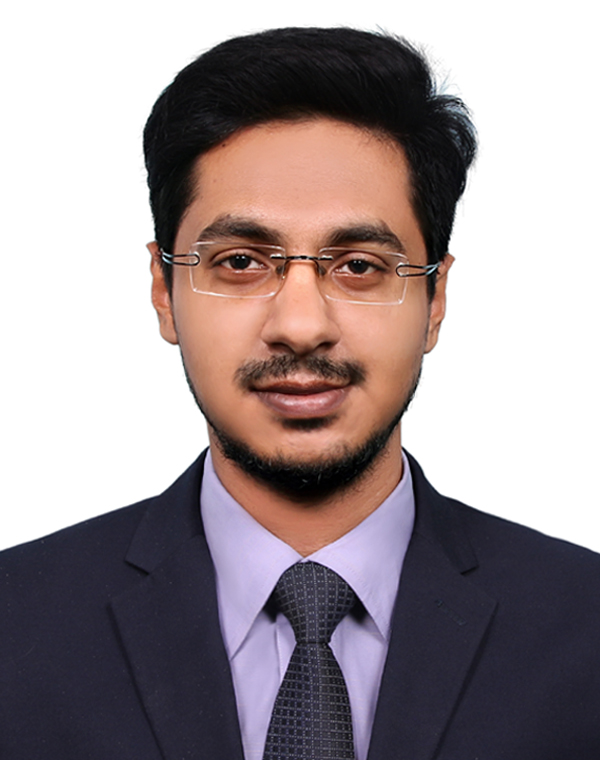
\includegraphics[width=3.5cm]{Dip.jpg}
\section{Address}
    GP-J-34
    Mohakhali,Gulshan
    Dhaka,1213
\section{Contact}
\href{Phone:+8801744499902}{Phone:01744499902}
\href{mail:dipghosh638@gmail.com}{dipghosh638@gmail}
\href{Github:https://github.com/Dip-Ghosh}{github://Dip-Ghosh}
\href{LinkedIn:https://www.linkedin.com/in/dip-ghosh-54b5aba3/}{LinkedIn://dip-ghosh/}
\href{http://facebook.com/dip638}{facebook://dip638}
\section{Programming
   Languages}
{\color{red} $\varheartsuit$}Laravel5.7
 {\color{red} $\varheartsuit$}C,C++
 JAVA
{\color{red} $\varheartsuit$}PHP
MVC(PHP)
JavaScript,Html5
 {\color{red} $\varheartsuit$}Bootstrap 4
AJAX,CSS3
JQuery
~
\section{Tecnology miscellaneous }
 {\color{red} $\varheartsuit$}Git,SVN
 Jira
 MySQL
 {\color{red} $\varheartsuit$}Oracle DataBase
  {\color{red} $\varheartsuit$}Latex
 Microsoft Office
\section{Programming Tools}
    Eclipse,phpStorm
    {\color{red} $\varheartsuit$}VSCode
    {\color{red} $\varheartsuit$}CodeBlocks
   MATLAB, Bracket
   {\color{red} $\varheartsuit$}Sublime,Atom,
   {\color{red} $\varheartsuit$} Latex
    {\color{red} $\varheartsuit$}Xampp,Wampp
    Microsoft Office
\end{aside}

\section{Career Objective}
To obtain a challenging and rewarding Software Engineer position where I can utilize my knowledge, proficiency, and skills to contribute to a company's growth.
\section{Education}
\begin{entrylist}
  \entry
    {2014-2018} 
    {B.SC. NORTH SOUTH UNIVERSITY}
    {Major in Computer Science and Engineering}
    {}
  \entry
    {2010-2012}
    {H.S.C.CANTT.PUBLIC SCHOOL AND COLLEGE,RANGPUR}
    {Major in Science}
        {}
  \entry
    {2001-2010}
    {S.S.C.THAKURGAON GOVT.BOYS' HIGH SCHOOL}
    {Major in Science}
     {}


%------------------------------------------------
\end{entrylist}
\section{Experience}
\begin{entrylist}
%------------------------------------------------
\entry
  {2019}
  {Roar IT Solutions}
  {February To April}
  {\jobtitle{Intern as a Web Developer}\\
  2.5 Months experience as Intern of PHP Developer in Roar IT Solutions}
  
%------------------------------------------------
\entry
  {2019-Present}
  {G8ICT Limited}
  {Monipuri Para,Dhaka}
  {\jobtitle{Junior Software Engineer}}

\end{entrylist}
\section{Projects}
\begin{entrylist}
%------------------------------------------------
\entry
{}
{RAB Project}
{{https://github.com/Dip-Ghosh/ProjectGovRab}}
{In the rab Project i have been working on Tender,NOC,Pages,login,news modules.I am basically doing the the crud operations like add,delete,update,view and show the work in the user pages.}
~
%------------------------------------------------
\end{entrylist}
\begin{entrylist}
\entry
{}
{Tulona Project }
{{https://github.com/Dip-Ghosh/Portal}}
{This is basically a web Portal using Laravel 5.8.In this web portal anyone can differentiate any type of item.Now i am working on the admin panel where Dynamic category,product can be added,deleted,updated,showed}

%------------------------------------------------
\end{entrylist}
\section{Varsity Project Details}

\begin{entrylist}
  \entry
    {Final Year}
    {Digital Scarecrow}
    {\href{https://github.com/Dip-Ghosh/An-Image-processing-based-digital-scarecrow}{http://github.com/Dip-Ghosh/An-Image-processing-based-digital-scarecrow}}
    {This is an image processing approach for digital scarecrow.The system is able to detect and track the pest birds from the real time video frame and from images. After the object is detected an alarm will raise as notification. The system can detect the bird with motion. The approach can implement in agricultural sector.}
  \entry
    {Third Year}
    {Online CloudShop}
    {\href{https://github.com/Dip-Ghosh/Online-CloudShop}{https://github.com/Dip-Ghosh/Online-CloudShop}}
    {This is a ecommerce site for buying and selling the product through online. The site is desinged so easily that anyone can access the daily necessary needs by a single click. Mainly Developed the \emph{Payment Method,Login,Cart etc}.}
  \entry
    {DataBase}
    {Cow-Hut}
    {\href{https://github.com/Dip-Ghosh/Cow-Hut}
    {https://github.com/Dip-Ghosh/Cow-Hut}}
    {In order to see the cattle anyone must have to logged in.Here the seller can add the cattle information only and other user just see the information of the cows and others and modify their details and so on.}
     \entry
    {Second Year}
    {Library management syetem}
    {\href{https://github.com/Dip-Ghosh/project}
    {https://github.com/Dip-Ghosh/project}}
    {In this project the student and the admin can login in borrow books and see the information.For this they have to logged in.The program is written in Java.}
 

\end{entrylist}
\clearpage
\begin{aside}
\section{Extra Curricular Activities}
~
      {\color{red} $\varheartsuit$} Photography
      Boyscouts
      Computer Club
      ~
\section{Languages}
~
    Bengali
    English
    ~
\section{Interest}
~
       {\color{red} $\varheartsuit$}Tamil Movies
      Cycling
      Portrait Photography
        {\color{red} $\varheartsuit$}Udemy Tutorial
      ~
\end{aside}
\vspace*{.7cm}
\section{Voluntary/Leadership Experience }
  { ICT And SCIENCE Tutor in Two different coaching centres and manage the  students by Ethical and moral values. }
      \\
    { Uttarer Ovijatrik is a Social service organzation where in winter we the member of this  organization help the poor people by giving the warm clothes and eid we try to help the Poor people by giving foods and new dresses.}
\begin{multicols}{2}
\section{Reference}

     {Tanzilur Rahman\\
     Assistant Professor & Program Coordinator\\
    Dept. of Electrical and Computer Engineering\\
    North South University\\
     Phone: +88 02 55668200 Ext – 6182\\
    Email: tanzilur.rahman@northsouth.edu\\}&&
   
    {Adnan Firoze\\
    Lecturer\\
    Dept. of Electrical and Computer Engineering\\
    North South University\\
    Phone: +88 02 55668200 Ext – 6187\\
    Email: adnan.firoze@northsouth.edu}\\
    
\end{multicols}
\end{document}